\chapter{Exercise 6}
\label{sec:ugeopgave-6}

The purpose of the exercise is to understand the principles of 2D texture mapping and how it can be used for polygon meshes. Furthermore, the purpose of the exercise is to understand the process of hidden surface removal and back-face culling

\section{Part 1}
\label{sec:del-1-1}

\subsection{Subpart a}
\label{subsec:del-1-a}
You can see the scene when hidden surface removal is disabled and enabled in Figure \ref{fig:6-1-1-1} and Figure \ref{fig:6-1-1-2}.
When hidden surface removal is enabled, the cube and left half of small polygon becomes invisible (we cannot see the difference occuring in small polygon because both big and small polygon is green).

\begin{figure}[hp]
\centering
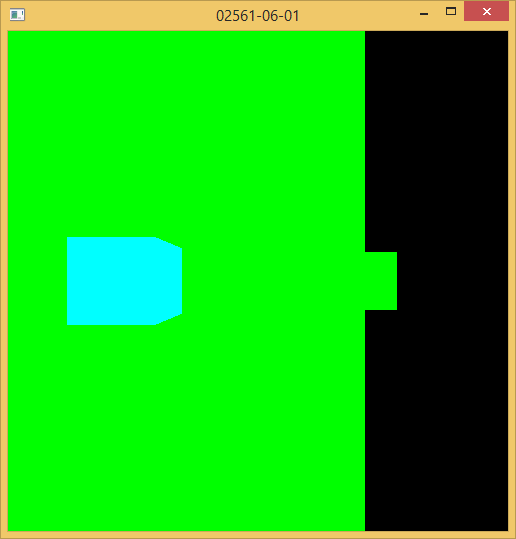
\includegraphics[width=8cm]{../Screenshots/ex-6/1a-1.png}
\caption{Hidden surface removal is disabled}
\label{fig:6-1-1-1}
\end{figure}

\begin{figure}[hp]
\centering
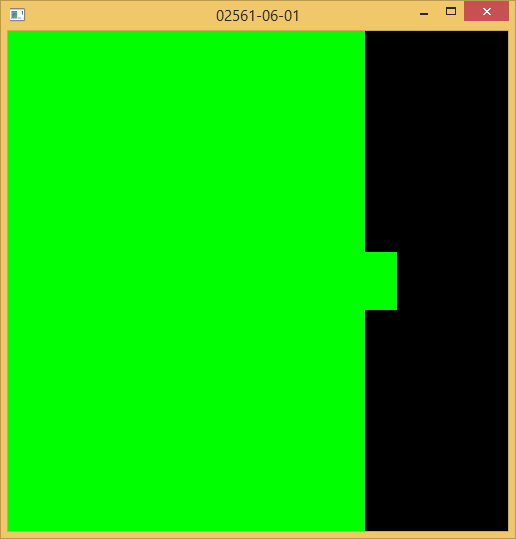
\includegraphics[width=8cm]{../Screenshots/ex-6/1a-2.png}
\caption{Hidden surface removal is enabled}
\label{fig:6-1-1-2}
\end{figure}

\subsection{Subpart b}
\label{subsec:del-1-b}

When GL\_BACK mode is activated (Figure \ref{fig:6-1-2-1}) , small polygon disappears. When GL\_FRONT mode is enabled (Figure  \ref{fig:6-1-2-2}), big polygon disappears. When GL\_FRONT\_AND\_BACK mode is activated (Figure  \ref{fig:6-1-2-3}), small and big polygon and the cube disappears.

\begin{figure}
        \centering
        \begin{subfigure}[b]{0.4\textwidth}
                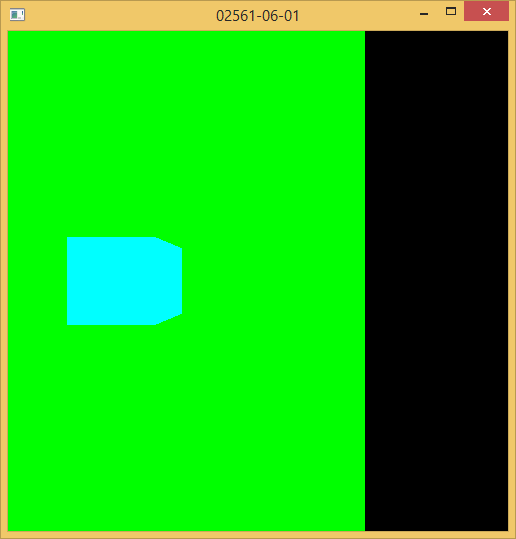
\includegraphics[width=6cm]{../Screenshots/ex-6/1b-1.png}
                \caption{GL\_BACK}
                \label{fig:6-1-2-1}
        \end{subfigure}

        \begin{subfigure}[b]{0.4\textwidth}
                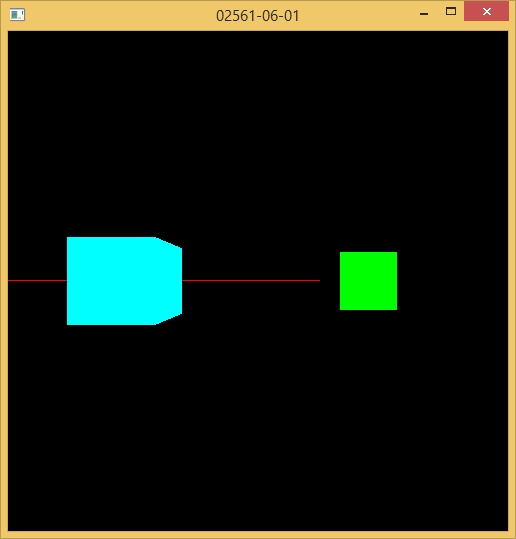
\includegraphics[width=6cm]{../Screenshots/ex-6/1b-2.png}
                \caption{GL\_FRONT}
                \label{fig:6-1-2-2}
        \end{subfigure}

        \begin{subfigure}[b]{0.4\textwidth}
                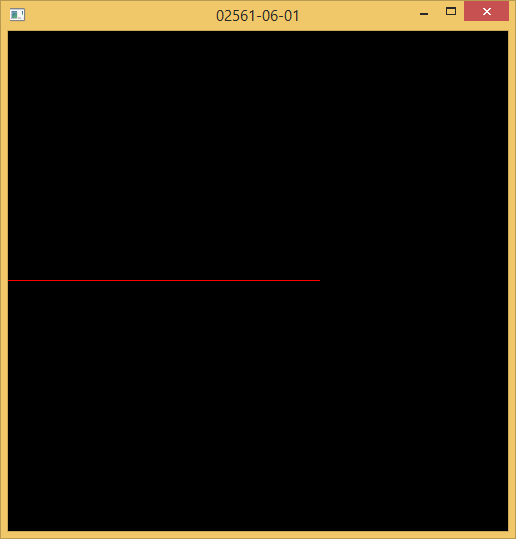
\includegraphics[width=6cm]{../Screenshots/ex-6/1b-3.png}
                \caption{GL\_FRONT\_AND\_BACK}
                \label{fig:6-1-2-3}
        \end{subfigure}
        \caption{Different face culling modes}\label{fig:6-1-2}
\end{figure}

\subsection{Subpart c}
\label{subsec:del-1-c}

If the angle between normal vector of a primitive and camera view direction is greater then 90 degrees, then the primitive is front facing. Otherwise, it is back facing.


\section{Part 2}
\label{sec:del-2-1}

I use the projection matrix given below.\\
\begin{lstlisting}
Perspective(24.3,WINDOW_WIDTH/(float)WINDOW_HEIGHT, 0.01, 10)
\end{lstlisting}

\smallskip
You can see resulting view of the scene in Figure \ref{fig:6-2}.

\begin{figure}[hp]
\centering
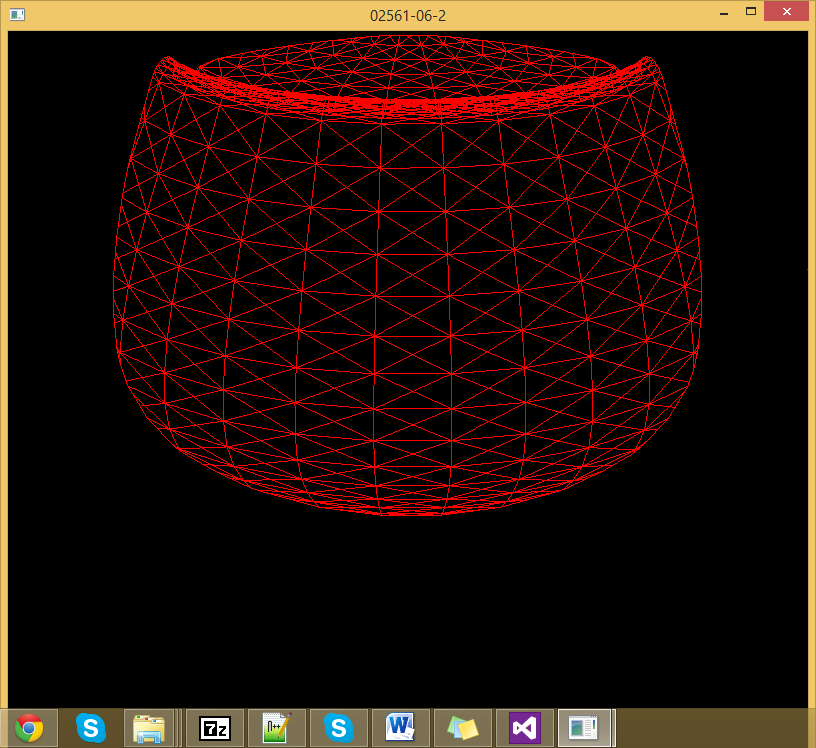
\includegraphics[width=8cm]{../Screenshots/ex-6/2.png}
\caption{Parts are clipped}
\label{fig:6-2}
\end{figure}

\section{Part 3}
\label{sec:del-3-1}


I implement keyboard functions which alters magnification and minification filters. You can see keyboard key mappings below.\\
Key 1 : Magnification filter is set to linear.\\
Key 2 : Magnification filter is set to nearest.\\
Key 3 : Minification filter is set to nearest mipmap nearest. \\
Key 4 : Minification filter is set to nearest mipmap linear. \\
Key 5 : Minification filter is set to nearest. \\
Key 6 : Minification filter is set to linear. \\
Key 7 : Minification filter is set to linear mipmap nearest. \\
Key 8 : Minification filter is set to linear mipmap linear. \\
Minification filter can be adjusted to six different modes. Magnification filter can be adjusted to two different modes. Therefore, for a single 2D texture, there are \emph{12} different combination of filters. Giving a sample and a screenshot for each combination in the report would spoil the flow of the report. This is because I prefer to give one example screenshot from these combinations see (Figure \ref{fig:6-3-1}). To see all possibilities, please navigate to program executable.

\begin{figure}[hp]
\centering
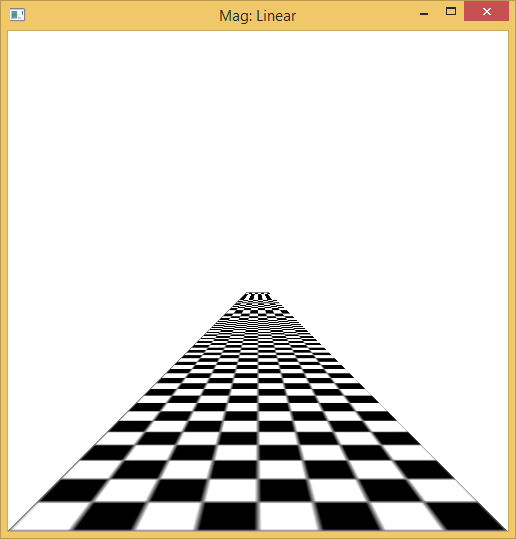
\includegraphics[width=8cm]{../Screenshots/ex-6/3-1.png}
\caption{Magnification and minification filters are both linear}
\label{fig:6-3-1}
\end{figure}



\section{Part 4}
\label{sec:del-4-1}

You can see all possible texture wrapping options below.

\begin{figure}[hp]
\centering
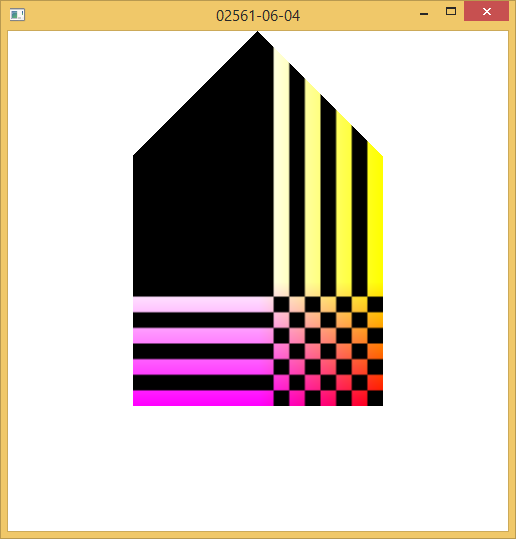
\includegraphics[width=8cm]{../Screenshots/ex-6/4-1.png}
\caption{GL\_TEXTURE\_WRAP\_T, GL\_REPEAT}
\label{fig:6-4-1}
\end{figure}

\begin{figure}[hp]
\centering
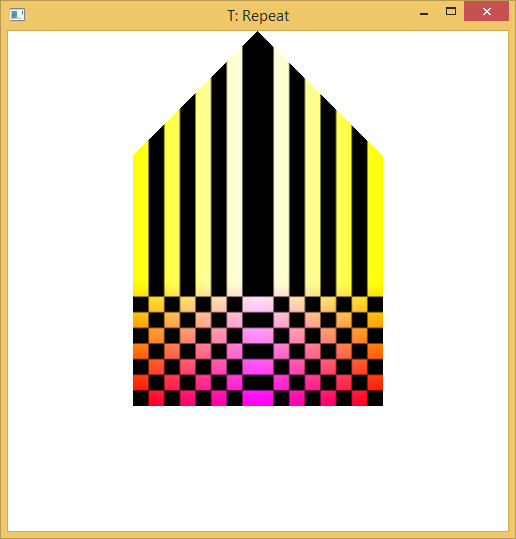
\includegraphics[width=8cm]{../Screenshots/ex-6/4-2.png}
\caption{GL\_TEXTURE\_WRAP\_T, GL\_MIRRORED\_REPEAT}
\label{fig:6-4-2}
\end{figure}

\begin{figure}[hp]
\centering
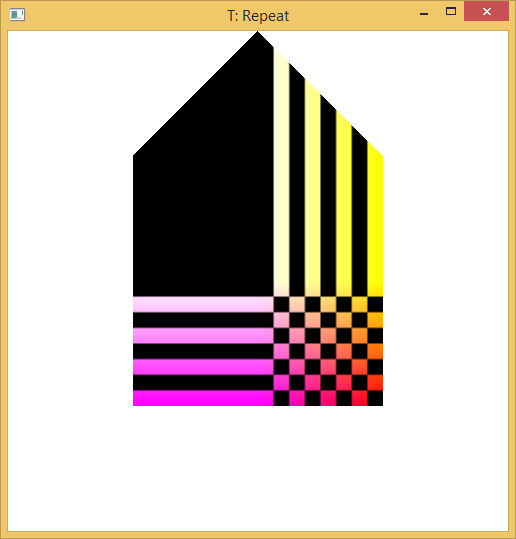
\includegraphics[width=8cm]{../Screenshots/ex-6/4-3.png}
\caption{GL\_TEXTURE\_WRAP\_T, GL\_CLAMP\_TO\_EDGE}
\label{fig:6-4-3}
\end{figure}


\begin{figure}[hp]
\centering
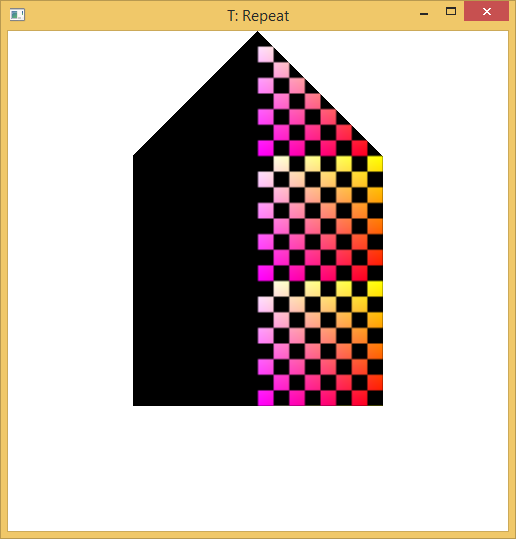
\includegraphics[width=8cm]{../Screenshots/ex-6/4-5.png}
\caption{GL\_TEXTURE\_WRAP\_S, GL\_REPEAT}
\label{fig:6-4-5}
\end{figure}

\begin{figure}[hp]
\centering
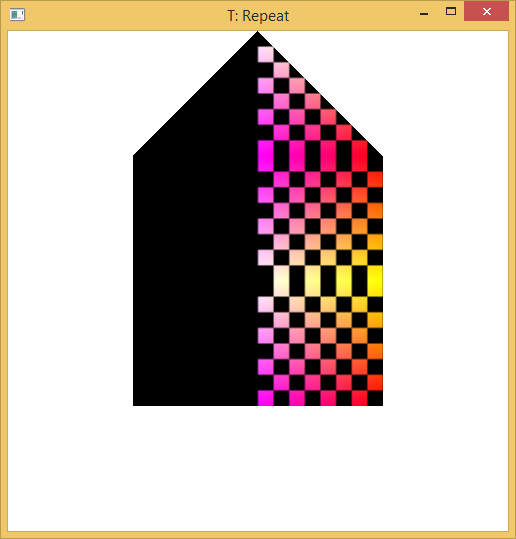
\includegraphics[width=8cm]{../Screenshots/ex-6/4-6.png}
\caption{GL\_TEXTURE\_WRAP\_S, GL\_MIRRORED\_REPEAT}
\label{fig:6-4-6}
\end{figure}

\begin{figure}[hp]
\centering
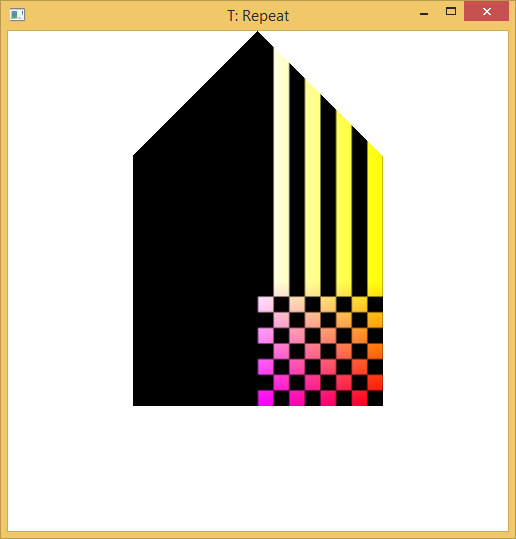
\includegraphics[width=8cm]{../Screenshots/ex-6/4-7.png}
\caption{GL\_TEXTURE\_WRAP\_S, GL\_CLAMP\_TO\_EDGE}
\label{fig:6-4-7}
\end{figure}


\section{Part 5}
\label{sec:del-5-1}

\begin{lstlisting}
vTextureCoord =(textureTrans *vec4(textureCoord,0.0,1.0)).xy;
\end{lstlisting}

This code piece is fetched from vertex shader. \emph{textureTrans} uniform matrix is multiplied with the extended vector of texture coordinates. Since \emph{textureTrans} is uniform, we can modify texture mapping in vertex shader.

\section{Part 6}
\label{sec:del-6-1}

I set \emph{idle} function as \emph{glutIdleFunc}. This is my implementation of \emph{idle} function: \\

\begin{lstlisting}
void idle()
{
	delta+=0.005;
	glutPostRedisplay();
}
\end{lstlisting}
The \emph{delta} float variable increases in each callback of idle function. \\
\emph{texturesTrans} uniform matrix is defined as: \\

\begin{lstlisting}
mat4 textureTrans=Translate(0.5, 0.5, 0.0) * RotateZ(delta) 
* Translate(-0.5, -0.5, 0.0);
\end{lstlisting}

It means textureTrans matrix is updated and changed periodically. In this way, I have an animation. To have a look at the animation that I create, please navigate to the executable program.
%%% Local Variables:
%%% mode: latex
%%% TeX-master: "report_main"
%%% End: 